% !TEX encoding = UTF-8
% !TEX TS-program = pdflatex
% !TEX root = ../tesi.tex

%**************************************************************
\chapter{Tecnologie utilizzate}
\label{cap3}

\section{Panoramica generale}
Durante la realizzazione del progetto sono state utilizzate le seguenti tecnologie e strumenti:

\subsubsection{Git} 
Git è un sistema di controllo di versione open source per la gestione di progetto di qualsiasi dimensione in maniera rapida ed efficiente. 

\subsubsection{Github}
GitHub è un servizi di hosting basato sul cloud che permette di gestire i progetti basati sul sistema di controllo versione Git. Oltre alle funzionalità di versionamento, offre funzionalità come issue tracking e continuous integration. 


\subsubsection{Python}
Python è un linguaggio di alto livello, general-purpose, dinamicamente tipizzato e garbage-collected. Nasce intorno al 1980 da Guido van Rossum, come sostituto del linguaggio di programmazione ABC. Per lo sviluppo del progetto è stata utilizzata la versione 3.9 del linguaggio.


\subsubsection{PyCharm Community Edition}
PyCharm Community Edition è un ambiente di sviluppo integrato open-source, specializzato nello sviluppo di progetti Python. Sviluppato da JetBrains, offre syntax highlighting, auto indentazione, code completion, controllo ortografia e un debugger Python built-in.

\subsubsection{\LaTeX}
\LaTeX{} è un linguaggio dichiarativo per la stesura di documenti. \'E stato usato per la
stesura dei vari documenti richiesti per il progetto di stage.


\subsubsection{StarUML}
StarUML è un software utilizzato per modellare diagrammi \gls{UML}.
\'E stato sviluppato da MKLabs ed è disponibile per Windows, Linux and MacOS.



\section{Analisi framework proposti}
\label{sec:analisi-framework}
\subsection{Dash}

\begin{figure}[H]
    \centering
    
\includegraphics[scale=0.4]{immagini/logo_dash.png}
   \caption{Logo Dash}
\end{figure}


Dash è un microframework open source sviluppato in Python annunciato nel 2017. Viene utilizzato per la visualizzazione dati e in generale per la creazione di applicazioni web per l'analisi dati.
Dash utilizza internamente le tecnologie Flask, Plotly.js e React.js.
\\
Un'app Dash è essenzialmente un'istanza di server Flask che comunica con i client tramite HTTP con pacchetti JSON, usando React.js per il front-end e in particolare sfrutta Plotly.js per la gestione dei grafici.

\subsubsection{Vantaggi e punti di forza}
Alcuni tra i punti di forza e vantaggi individuati sono:
\begin{itemize}
\item Non richiede l'utilizzo di HTML/CSS o Javascript aggiuntivi, in quanto ogni componente in Dash codifica tutte le proprietà di uno specifico componente di React;
\\
Sono infatti presenti classi Python che codificano la maggior parte dei tag HTML (tramite \textit{dash\_html\_component}) e tutti i componenti interattivi di base offerti da React (Slider, Dropdown, Graph, ...), tramite \textit{dash\_core\_components} \cite{site:dash-core-comp};

\item Dash supporta l'aggiunta di nuovi componenti, creando un oggetto sopra a componenti preesistenti in React o definendo un proprio componente personalizzato tramite HTML/CSS e Javascript;

\item Pur facendo uso di fogli di stile di default, supporta l'aggiunta di fogli di stile CSS esterni, quindi ogni elemento è personalizzabile usando le \gls{API} offerte da Dash, oppure introducendo i propri fogli di stile, garantendo il massimo livello di personalizzazione possibile;

\item Il codice è dichiarativo e reattivo, e questo semplifica molto lo sviluppo di applicazioni (anche complesse) con numerosi componenti interattivi;

\item L'istanza di Flask alla base del server, resta totalmente accessibile, permettendo la modifica di tutte le sue proprietà configurabili. Inoltre può essere estesa (a seconda dei bisogni) con tutta una serie di plugin Flask;

\item Ottima visualizzazione degli errori per il debugging; in particolare non vengono nascosti nella console Javascript, ma evidenziati nelle grafica dell'applicazione, quando è in modalità di debug. Vengono anche isolati dalle eccezioni generate da Flask internamente, permettendo una netta distinzione tra un errore causato da Flask o da Dash;

\item Tracciamento efficace delle callback; Dash crea una visualizzazione grafica dell'albero delle callback, indicando quando sono state eseguite, per quanto hanno operato e i dati che sono stati passati.
Questo si prova molto utile, soprattutto in applicazioni medio-grandi, dove il numero di callback può diventare notevole rapidamente;

\item Dash salva lo stato dell'applicazione nel client, cioè nel browser, questo permette di avere dashboard che supportano più utenti in simultanea, permettendo di avere interazioni indipendenti con la stessa applicazione e riducendo le risorse necessarie per un nuovo utente dal lato server;

\item La presenza di più community attive e molto materiale informatico e formativo, all'infuori della documentazione;

\item Molto utilizzato e riconosciuto in ambito aziendale, tanto da offrire un'opzione premium a pagamento, Dash Enterprise.

\end{itemize}

\subsubsection{Svantaggi e punti di debolezza}
Alcuni tra i punti di debolezza individuati sono:
\begin{itemize}
\item L'aggiornamento costante di elementi grafici può diventare rapidamente oneroso vista l'architettura sopra la quale è sviluppato, dato che non avendo una cache lato server vanno comunque rifatti tutti i calcoli necessari anche se i dati non sono cambiati;

\item Dash rimane molto chiuso ad integrazioni con altre librerie grafiche, dato che per design l'unica supportata rimane Plotly.js, questo può essere limitante a seconda delle applicazioni;

\item La creazione di applicazioni multi pagina è stata resa disponibile di recente (prima non era esplicitamente supportata e c'era il bisogno di sviluppare soluzioni non standard e poco stabili), e rimane limitata. Ad esempio lo scambio di dati tra le pagine dell'applicazione deve essere sviluppato esplicitamente (visto che Dash è stateless) e può diventare complesso in poco tempo e provocare una riduzione delle performance;

\item L'interattività offerta da Dash, seppur funzionale e concisa, rimane limitata, sia per opzioni (solo callback collegate a cambi di proprietà dei componenti) che per funzionalità, per esempio non è possibile che due o più callback aggiornino lo stesso elemento. 
\\
Questo può portare a soluzioni macchinose e poco eleganti (passaggio di argomenti aggiuntivi come identificativi e definire una grande callback che accetta tutti gli input e output e con una logica complessa per ritornare la risposta corretta, mescolando comportamenti e funzionalità logicamente separate tra di loro);


\item Può richiedere conoscenze rudimentali di HTML (e CSS per un design "grafico" migliore e personalizzazione maggiore). Non sono strettamente necessarie, finché la dimensione dell'applicazione che si vuole sviluppare rimane ridotta, però con il crescere di quest'ultima possono diventarlo. A queste si aggiunge la necessità di conoscere Javascript se si vuole deviare dai comportamenti standard dei componenti;

\item In generale, anche dovuto a quanto detto nel punto sopra, lo sviluppo in Dash può diventare complesso, soprattutto appena ci si sposta su layout più complicati;

\item Difficoltà nel deployment, dato che per un'applicazione Dash il deploy avviene solo nelle piattaforme che supportano Flask, inoltre necessita un setup non triviale dell'ambiente di esecuzione, e su questi aspetti la documentazione è scarsa;

\item Dash non supporta molte funzionalità relative all'accessibilità per la maggior parte dei componenti di default offerti e per i grafici renderizzati con Plotly.js.
	
\end{itemize}

\subsection{Panel}

\begin{figure}[H]
    \centering
    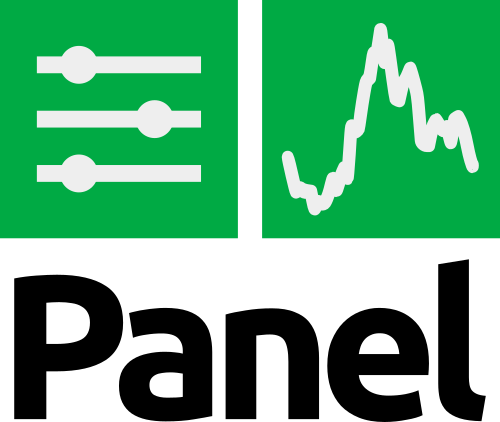
\includegraphics[scale=0.4]{immagini/logo_panel.png}
   \caption{Logo Panel}
\end{figure}


Panel è una libreria Python open source, annunciata nel maggio del 2019, che permette di creare applicazioni web interattive e dashboard personalizzate.
Panel è costruito sopra due librerie principali: 
\begin{itemize}
	\item Bokeh, un framework che implementa il pattern MVC su cui si basa Panel; offre anche alcuni componenti base, un layout manager e un server Tornado per la comunicazione tra Python e browser (usando Websocket);
	
	\item Param, un framework per definire parametri reattivi, usati per definire tutti i componenti di Panel.

\end{itemize}

\subsubsection{Vantaggi e punti di forza}
Alcuni tra i punti di forza e vantaggi individuati sono:
\begin{itemize}
\item Panel è stato pensato per essere utilizzato puramente in Python, rendendo non necessaria neanche una minima conoscenza di HTML/CSS e Javascript;

\item Panel può interfacciarsi con praticamente tutte le librerie di plotting più comuni (es. Plotly.js, matplotlib, ...);

\item Panel si interfaccia nativamente anche con molti degli strumenti connessi all'analisi dati (es. Pandas, Dusk, Datashader, ...);

\item Ottimo supporto per la creazione di applicazioni multi-pagina, tramite l'utilizzo di Pipelines, che permettono la facile definizione di un workflow, dove lo stadio precedente passa i dati allo stadio successivo;

\item Offre potenti \gls{API} per i bisogni di ogni sviluppatore \cite{site:panel-apis}:
	\begin{itemize}
		\item Interact functions: genera un'interfaccia grafica in automatico, data una funzione (la più semplice ma meno personalizzabile);
		
		\item Reactive functions: simile ad Interact functions, ma richiede che i componenti siano dichiarati in maniera esplicita e che i collegamento tra componenti e funzioni sia esplicito;
		
		\item Parameterized classes: tramite Param, permette di definire classi parametrizzate (dove vengono dichiarati i parametri e i loro intervalli), indipendenti dall'interfaccia grafica, che sarà poi generata da Panel. Questo determina molte ottimizzazioni e soprattutto una funzionalità di validazione dei parametri già pronta all'uso (tramite Param);
		
		\item Callbacks: l'interfaccia grafica viene generata dichiarando tutti i componenti necessari e ogni callback necessaria per interazione e l'aggiornamento (il metodo più "vicino" alla macchina, quindi più complesso ma più personalizzabile).
	
	\end{itemize}
	
Questo determina un elevato grado di flessibilità di sviluppo;

\item L'architettura su cui Panel è costruito salva lo stato per ogni utente e sessione sia nel server che nel client (browser) e se necessario è possibile sincronizzarli. Questo ha importanti implicazioni, permette infatti di salvare in una cache lato server le computazioni intermedie per ogni utente e rende l'applicazione molto più responsive, permettendo un'esplorazione continua di una visualizzazione con rallentamenti anche impercettibili, perché vengono ricalcolati solo i passaggi necessari; 

\item Panel renderizza l'applicazione tramite l'utilizzo di un template di default ma offre la possibilità di inserire nuovi template personalizzati e sviluppati dall'utente, permettendo il controllo sul layout di ogni singolo componente.

\end{itemize}



\subsubsection{Svantaggi e punti di debolezza}
Alcuni tra i punti di debolezza individuati sono:
\begin{itemize}
\item L'architettura sulla quale è sviluppato non scala molto bene se l'applicazione richiede di supportare una molteplicità di utenti simultanei, in quanto può velocemente saturare le risorse del server;

\item Similmente a Dash, la difficoltà di utilizzo aumenta di molto se le applicazioni e i layout diventano più complessi. In generale Panel ha una curva di apprendimento più complessa rispetto a Dash;

\item La quantità di materiale informativo e formativo disponibile (non considerando la documentazione) è considerevolmente minore rispetto a Dash. Alcuni dei motivi sono il fatto che Dash è uscito 2 anni prima di Panel, e vista la presenza di Dash Enterprise, si è venuta a una comunità più numerosa;

\item L'attività di debugging viene resa più complessa (rispetto a Dash) per la mancanza di un interfaccia chiara per la visualizzazione degli errori che sono mostrati nella console Javascript come errori o eccezioni delle librerie interne al framework. Questo rende più difficile, rispetto a Dash, la comprensione di cosa causa l'errore in caso essi siano non triviali. Di recente è stata introdotta un Debugging widget, che pur mitigando il problema resta limitata;

\item Difficoltà nel deployment, dove Panel ha comunque un numero più vasto di piattaforme sulla quale si può effettuare il deploy, resta il problema della scarsa documentazione, che manca di profondità (le varie opzioni sono discusse solo brevemente);

\item La presenza di molteplici \gls{API} di sviluppo può portare (soprattutto degli sviluppatori alle prime armi con il framework) ad effettuare delle scelte sbagliate, richiedendo in un tempo successivo un grande sforzo di refactoring.

\end{itemize}

\subsection{Scelta framework e motivazioni}
In accordo con il proponente, è stato scelto di utilizzare il framework Dash. In un primo momento si era deciso di usare Panel, ma lo sviluppo di un piccolo \gls{PoC} ha reindirizzato la scelta.
\\
In particolare le motivazioni (alcune personali) sono:
\begin{itemize}
\item Difficoltà nel debugging di Panel rispetto a Dash: come spiegato sopra, il fatto che Panel visualizzi principalmente gli errori e le eccezioni delle librerie interne, rendeva il processo di individuazione dei bug inevitabilmente lungo e tedioso. Ho invece trovato l'interfaccia offerta da Dash per la visualizzazione delle eccezioni più chiara e diretta, senza contare l'utilità delle mappa grafica dell'esecuzione delle callback generata da Dash, che invece in Panel era completamente assente;

\item Alcuni punti di debolezza di Dash sono stati mitigati, tramite le Dash Extensions \cite{site:dash-ext}. In particolare il \texttt{MultiplexerTransform}, che permette di definire più callback con lo stesso output, migliorando la definizione delle callback e permettendo la suddivisione delle funzionalità;

\item La scarsa presenza di materiare formativo e informativo per Panel e la ridotta documentazione rispetto a Dash, è stata forse la motivazione che ha avuto più impatto nella scelta del framework. Infatti la presenza di un ottimo forum \cite{site:dash-forum}, di numerose guide online e di componenti aggiuntivi non standard già sviluppati si sono rivelati di fondamentale importanza e utilità.

\end{itemize}
